%=====================================================================
%  ERP-CONTRACTOR - QHSE OPERATIONS PLATFORM  --  TECHNICAL SOFTWARE REPORT
%  Compiles with pdfLaTeX on Overleaf. No external images required;
%  every figure is drawn in TikZ.
%=====================================================================
\documentclass[11pt]{article}

\usepackage[letterpaper,margin=1in]{geometry}
\usepackage{lmodern}
\usepackage[T1]{fontenc}
\usepackage[utf8]{inputenc}
\usepackage[dvipsnames]{xcolor}
\usepackage{tikz}
\usetikzlibrary{positioning,calc,arrows.meta,shapes.geometric,fit,backgrounds}
\usepackage{graphicx}
\usepackage{booktabs}
\usepackage{array}
\usepackage{float}
\usepackage{enumitem}
\usepackage{titlesec}
\usepackage{fancyhdr}
\usepackage{caption}
\usepackage{amsmath,amssymb}
\usepackage[hidelinks]{hyperref}

%----------------------------- palette -------------------------------
\definecolor{reportblue}{RGB}{45,78,112}
\definecolor{inkgray}{RGB}{85,85,85}
\definecolor{linegray}{RGB}{150,150,150}
% app (dark theme) palette for the UI figure
\definecolor{apbg}{HTML}{0B1220}
\definecolor{apsurface}{HTML}{111A2E}
\definecolor{apsurf2}{HTML}{1B2740}
\definecolor{aptext}{HTML}{E6EDF7}
\definecolor{apmuted}{HTML}{93A1B5}
\definecolor{apblue}{HTML}{3B82F6}
\definecolor{apgreen}{HTML}{22C55E}
\definecolor{apamber}{HTML}{F59E0B}
\definecolor{apred}{HTML}{EF4444}
\definecolor{apborder}{HTML}{25324A}

%----------------------------- styling -------------------------------
\titleformat{\section}{\Large\bfseries\color{reportblue}}{\thesection}{0.7em}{}
\titleformat{\subsection}{\large\bfseries\color{inkgray}}{\thesubsection}{0.6em}{}
\titlespacing*{\section}{0pt}{1.6em}{0.7em}
\captionsetup{font=small,labelfont={bf,color=reportblue}}
\setlist{itemsep=2pt,topsep=3pt}

\pagestyle{fancy}
\fancyhf{}
\fancyhead[L]{\small\color{inkgray}\scshape ERP-Contractor --- QHSE Operations Platform}
\fancyhead[R]{\small\color{inkgray}\thepage}
\renewcommand{\headrulewidth}{0.4pt}
\renewcommand{\headrule}{\hbox to\headwidth{\color{linegray}\leaders\hrule height \headrulewidth\hfill}}

% helper for a KPI card inside the dashboard figure: {x}{y}{label}{value}{color}
\newcommand{\kpicard}[5]{%
  \fill[apsurf2,rounded corners=2pt] (#1,#2) rectangle ++(3.35,1.7);
  \node[anchor=north west,text=apmuted,font=\scriptsize] at (#1+0.18,#2+1.53) {#3};
  \node[anchor=north west,text=#5,font=\large\bfseries] at (#1+0.16,#2+1.02) {#4};
}

\begin{document}

%=====================================================================
%  TITLE PAGE
%=====================================================================
\begin{titlepage}
\thispagestyle{empty}
\centering
\vspace*{0.6cm}

{\scshape\Large\color{reportblue} Technical Software Report}\\[0.35em]
{\scshape\color{inkgray} QHSE $\cdot$ Compliance $\cdot$ Full-Stack Engineering}\\[0.7em]
{\color{black}\rule{\textwidth}{1.3pt}}\\[0.7cm]

{\fontsize{40}{46}\selectfont\bfseries ERP-Contractor}\\[0.35cm]
{\Large A Local-First QHSE Operations Platform}\\[0.28cm]
{\large\itshape Systems Design, Data Architecture, Compliance Engine, and Reporting}\\[0.55cm]
{\color{black}\rule{\textwidth}{0.6pt}}\\[0.9cm]

% ---------------- cover schematic (wireframe) ----------------
\resizebox{0.9\textwidth}{!}{%
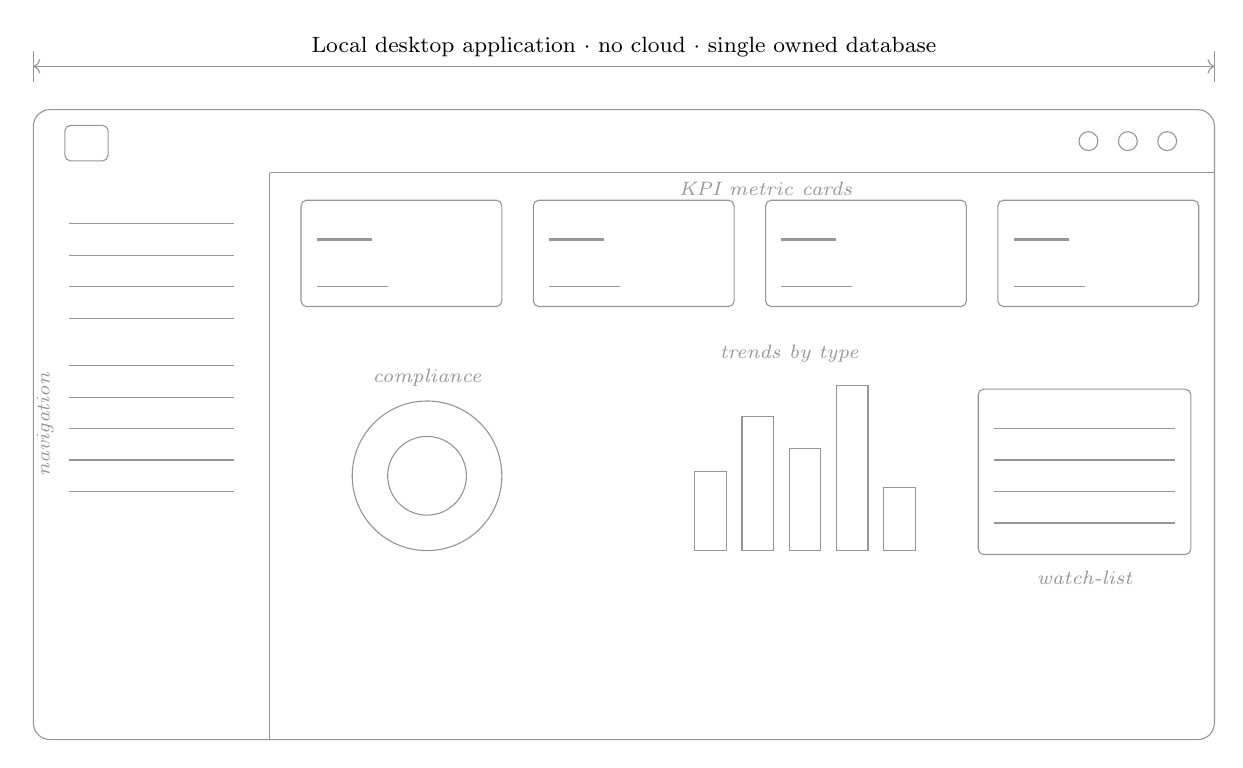
\begin{tikzpicture}[line width=0.4pt]
  \colorlet{lg}{linegray}
  % top dimension line
  \draw[<->,lg] (0,8.55) -- node[above,black,font=\footnotesize]{Local desktop application $\cdot$ no cloud $\cdot$ single owned database} (15,8.55);
  \draw[lg] (0,8.35)--(0,8.75); \draw[lg] (15,8.35)--(15,8.75);
  % window
  \draw[lg,rounded corners=6pt] (0,0) rectangle (15,8);
  \draw[lg] (3,0)--(3,7.2);          % sidebar divider
  \draw[lg] (3,7.2)--(15,7.2);       % top bar
  % logo + nav
  \draw[lg,rounded corners=2pt] (0.4,7.35) rectangle ++(0.55,0.45);
  \foreach \y in {6.55,6.15,5.75,5.35,4.75,4.35,3.95,3.55,3.15}{\draw[lg] (0.45,\y)--(2.55,\y);}
  \node[lg,font=\scriptsize,rotate=90] at (0.15,4){\itshape navigation};
  % top bar controls
  \foreach \x in {13.4,13.9,14.4}{\draw[lg] (\x,7.6) circle (0.12);}
  % KPI cards (two rows of four)
  \foreach \x in {3.4,6.35,9.3,12.25}{
     \draw[lg,rounded corners=2pt] (\x,5.5) rectangle ++(2.55,1.35);
     \draw[lg] (\x+0.2,5.75)--(\x+1.1,5.75);
     \draw[lg,line width=1.2pt] (\x+0.2,6.35)--(\x+0.9,6.35);
  }
  \node[lg,font=\scriptsize] at (9.3,7.0){\itshape KPI metric cards};
  % charts row
  \draw[lg] (5.0,3.35) circle (0.95);
  \draw[lg] (5.0,3.35) circle (0.5);
  \foreach \x/\h in {8.4/1.0,9.0/1.7,9.6/1.3,10.2/2.1,10.8/0.8}{\draw[lg] (\x,2.4) rectangle ++(0.4,\h);}
  \node[lg,font=\scriptsize] at (5.0,4.6){\itshape compliance};
  \node[lg,font=\scriptsize] at (9.6,4.9){\itshape trends by type};
  % watchlist
  \draw[lg,rounded corners=2pt] (12.0,2.35) rectangle ++(2.7,2.1);
  \foreach \y in {2.75,3.15,3.55,3.95}{\draw[lg] (12.2,\y)--(14.5,\y);}
  \node[lg,font=\scriptsize] at (13.35,2.05){\itshape watch-list};
\end{tikzpicture}}\par
\vspace{0.35cm}
{\small\itshape General arrangement of the primary dashboard (schematic, not a live capture).}

\vfill
{\color{black}\rule{\textwidth}{0.6pt}}\\[0.5cm]
\begin{tabular}{@{}>{\bfseries\color{black}}l l@{}}
Author: & Salman K. Alwajaan\\[2pt]
Contact: & Salman.khalid.alwajaan@gmail.com\\[2pt]
Document: & Revision 1.0 \quad$\cdot$\quad 2026\\
\end{tabular}
\vspace*{0.4cm}
\end{titlepage}

%=====================================================================
%  ABSTRACT + TOC
%=====================================================================
\begin{abstract}
\noindent ERP-Contractor is a locally hosted, single-owner software platform that unifies the
Quality, Health, Safety, Environment (QHSE) and human-resources operations of a small
electrical-contracting company. It replaces a fragmented collection of spreadsheets with
one relational database and a dynamic desktop interface, eliminating manual reconciliation
while adding proactive compliance monitoring. This report documents the platform's design
goals, software architecture, relational data model, functional modules, the tag-based
(NFC / QR) inspection system, PPE inventory and storage, the credential
compliance (expiry) engine, spreadsheet interoperability, security and data-ownership model,
and verification results. The system is implemented as an Electron desktop application
(React user interface) backed by an embedded SQLite database, and runs entirely offline on
a single laptop with no cloud dependency or subscription.
\end{abstract}

\tableofcontents
\newpage

%=====================================================================
\section{Introduction}
\subsection{Background and Problem Statement}
The company operates as a contractor for a national electrical utility. Critical operational
data --- employee records, professional licenses, training courses, government and client-issued
identity cards (Iqama, Industrial Security Cards, Municipality permits), personal protective
equipment (PPE), daily safety inspections, ISO documentation, environmental logs, quality
records, and project work orders --- was historically distributed across numerous, disconnected
Excel files. This manual model is time-consuming, error-prone, and offers no real-time
visibility. Because the utility client mandates weekly updates of employee data and because
lapsed credentials carry regulatory and contractual risk, the absence of a single source of
truth is a direct operational liability.

\subsection{Objectives}
\begin{itemize}
  \item Consolidate all QHSE and HR data into one relational database (a single source of truth).
  \item Provide a fast, modern, desktop interface --- explicitly not a generic spreadsheet clone.
  \item Track every expiring credential automatically and surface it before it lapses.
  \item Preserve full data ownership: local storage, offline operation, no subscription.
  \item Interoperate with the existing Excel workflow through structured import and export.
  \item Extend beyond safety to dedicated Environment and Quality departments.
\end{itemize}

\subsection{Scope}
This document covers the delivered version~1.0 of the platform: its architecture, data model,
modules, and operation. Hardware integration for physical NFC tags (a mobile-companion concern)
and a signed, packaged application binary are identified as future work in Section~\ref{sec:future}.

%=====================================================================
\section{System Overview}
\subsection{Design Goals}
Four properties drove every design decision: (i)~\textbf{local-first} --- the application and its
data reside on the user's machine; (ii)~\textbf{owned} --- data is stored in an open, portable
database file the user controls; (iii)~\textbf{powerful UI} --- a dynamic, themeable interface
with charts and drill-down, in both dark and bright modes; and (iv)~\textbf{single platform} ---
one integrated system rather than a patchwork of tools.

\subsection{Technology Stack}
\begin{table}[H]
\centering\small
\begin{tabular}{@{}l l l@{}}
\toprule
\textbf{Layer} & \textbf{Technology} & \textbf{Role} \\
\midrule
Desktop shell     & Electron              & Native window, offline runtime, OS integration \\
User interface    & React + Vite          & Dynamic, component-based front end \\
Styling / theming & Tailwind CSS          & Design tokens, dark / bright mode \\
Charts            & Recharts              & KPI donut, trend and bar visualizations \\
Database          & SQLite (via sql.js)   & Embedded relational store, single file \\
Spreadsheets      & ExcelJS               & Excel / CSV import and export \\
\bottomrule
\end{tabular}
\caption{Implementation stack. The SQLite engine is compiled to WebAssembly, avoiding native
build steps while remaining a genuine relational database.}
\end{table}

%=====================================================================
\section{Software Architecture}
\subsection{Process Model}
The application follows Electron's isolated three-part model. The \emph{renderer} hosts the React
interface and never touches the database or file system directly. A \emph{preload} bridge exposes a
single, narrow, contextually isolated function to the interface. The \emph{main} process owns the
database, the file system, and all native dialogs. This separation is a security boundary: the
interface can only request data through one audited channel.

\begin{figure}[H]
\centering
\resizebox{0.98\textwidth}{!}{%
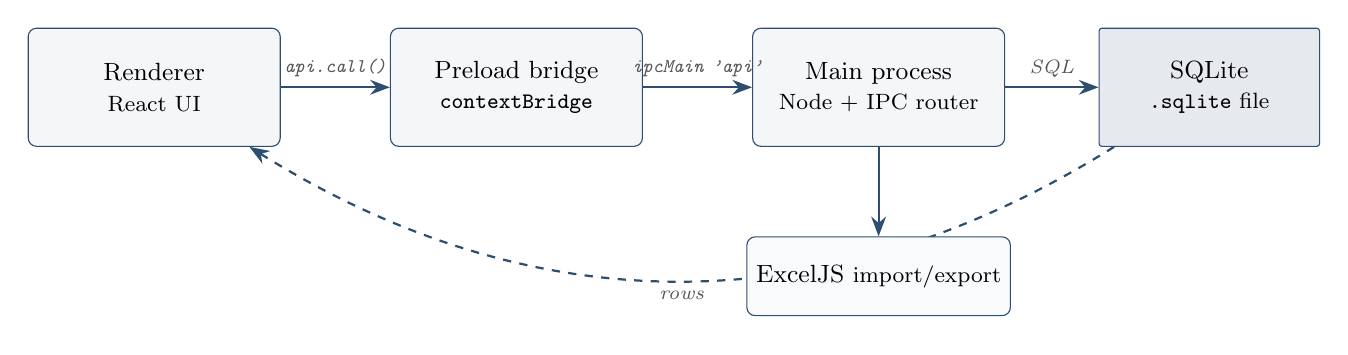
\begin{tikzpicture}[
   box/.style={draw=reportblue,rounded corners=3pt,fill=reportblue!5,minimum height=1.5cm,
               minimum width=3.2cm,align=center,font=\small},
   store/.style={draw=reportblue,fill=reportblue!12,rounded corners=1pt,minimum height=1.5cm,
               minimum width=2.8cm,align=center,font=\small},
   lbl/.style={font=\scriptsize\itshape,color=inkgray},
   arr/.style={-{Stealth[length=2.5mm]},thick,color=reportblue}]
  \node[box] (r) at (0,0) {Renderer\\ \footnotesize React UI};
  \node[box] (p) at (4.6,0) {Preload bridge\\ \footnotesize \texttt{contextBridge}};
  \node[box] (m) at (9.2,0) {Main process\\ \footnotesize Node + IPC router};
  \node[store] (db) at (13.4,0) {SQLite\\ \footnotesize \texttt{.sqlite} file};
  \draw[arr] (r) -- node[lbl,above]{\texttt{api.call()}} (p);
  \draw[arr] (p) -- node[lbl,above]{\texttt{ipcMain} \texttt{'api'}} (m);
  \draw[arr] (m) -- node[lbl,above]{SQL} (db);
  \draw[arr,dashed] (db) to[bend left=32] node[lbl,below]{rows} (r);
  \node[box,minimum width=2.6cm,minimum height=1cm,fill=reportblue!3] (x) at (9.2,-2.4)
        {ExcelJS \footnotesize import/export};
  \draw[arr] (m) -- (x);
\end{tikzpicture}}
\caption{Process architecture. All data flows through one inter-process channel; the renderer has
no direct database or file-system access.}
\end{figure}

\subsection{The Data Channel}
Every operation is expressed as a single call of the form \texttt{call(action, params)} where
\texttt{action} is a dotted string such as \texttt{employees.list} or \texttt{licenses.create}. The
main process routes the action to a generic create/read/update/delete engine or to a specialised
handler (dashboard aggregation, compliance scan, Excel transfer). This uniformity keeps the surface
area small and every write auditable.

\subsection{Persistence}
The database is a single SQLite file stored in the operating system's per-user application-data
directory. After each mutation the engine serialises the full database to disk, guaranteeing
durability; the identifier of a newly inserted row is captured before serialisation. Backing up the
system is a single file copy.

%=====================================================================
\section{Data Model}
\subsection{Relational Schema}
The schema is normalised around a central \texttt{employees} table. Each employee is the anchor for
their licenses, cards, courses and issued PPE, linked by the business key \texttt{emp\_id}. Project
work, environmental records and quality reports form a second cluster linked by project. Joined
database \emph{views} carry human-readable names (employee, project) into list queries so the
interface never needs to resolve foreign keys itself.

\begin{table}[H]
\centering\small
\begin{tabular}{@{}l p{7.2cm} l@{}}
\toprule
\textbf{Table} & \textbf{Purpose} & \textbf{Key link} \\
\midrule
\texttt{employees}          & Master personnel records (single source of truth) & --- \\
\texttt{id\_cards}          & Iqama, Industrial Security, Municipality, etc.     & \texttt{emp\_id} \\
\texttt{licenses}           & Professional / operating licenses with expiry      & \texttt{emp\_id} \\
\texttt{courses}            & Completed training and certifications              & \texttt{emp\_id} \\
\texttt{ppe\_items}         & PPE catalogue and stock levels                     & --- \\
\texttt{ppe\_issues}        & PPE assigned to an employee (with acknowledgment)  & \texttt{emp\_id} \\
\texttt{assets}             & Job sites, vehicles, equipment (NFC / QR tags)     & --- \\
\texttt{inspections}        & Daily inspections with checklist and score         & \texttt{asset\_id} \\
\texttt{documents}          & Controlled ISO documents (45001 / 14001 / 9001)    & --- \\
\texttt{document\_versions} & Version history for each document                  & \texttt{document\_id} \\
\texttt{projects}           & Contracts, orders and study projects               & --- \\
\texttt{tasks}              & Work orders and assignments                        & \texttt{project\_id} \\
\texttt{environment\_records}& Cooling-oil pulls, staking returns, waste removal & \texttt{project\_id} \\
\texttt{quality\_ncr}       & Non-conformance reports and corrective actions     & \texttt{project\_id} \\
\texttt{quality\_audits}    & Internal / external / certification audits         & --- \\
\texttt{audit\_log}         & Immutable record of every create / update / delete & --- \\
\bottomrule
\end{tabular}
\caption{Core relational tables. Reference tables (users, settings) are omitted for brevity.}
\end{table}

\subsection{Entity Relationships}
\begin{figure}[H]
\centering
\resizebox{0.95\textwidth}{!}{%
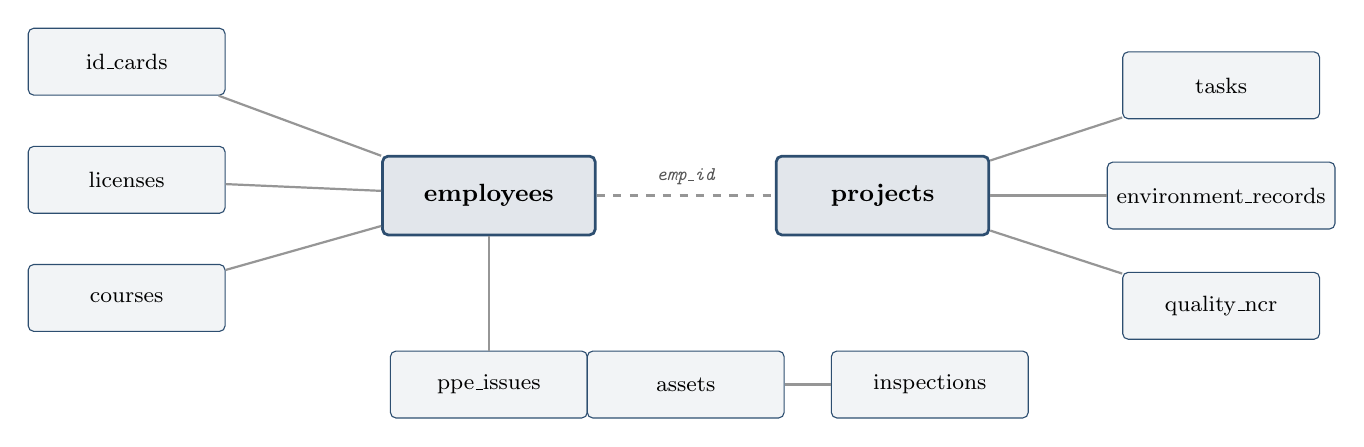
\begin{tikzpicture}[
  ent/.style={draw=reportblue,rounded corners=2pt,fill=reportblue!6,minimum width=2.5cm,
              minimum height=0.85cm,align=center,font=\footnotesize},
  hub/.style={draw=reportblue,line width=1pt,fill=reportblue!14,rounded corners=2pt,
              minimum width=2.7cm,minimum height=1cm,align=center,font=\small\bfseries},
  rel/.style={color=linegray,thick}]
  \node[hub] (emp) at (0,0) {employees};
  \node[ent] (cards) at (-4.6,1.7) {id\_cards};
  \node[ent] (lic)   at (-4.6,0.2) {licenses};
  \node[ent] (crs)   at (-4.6,-1.3) {courses};
  \node[ent] (ppe)   at (0,-2.4) {ppe\_issues};
  \draw[rel] (emp) -- (cards); \draw[rel] (emp) -- (lic);
  \draw[rel] (emp) -- (crs);   \draw[rel] (emp) -- (ppe);
  \node[hub] (prj) at (5,0) {projects};
  \node[ent] (tsk) at (9.3,1.4) {tasks};
  \node[ent] (env) at (9.3,0) {environment\_records};
  \node[ent] (ncr) at (9.3,-1.4) {quality\_ncr};
  \draw[rel] (prj) -- (tsk); \draw[rel] (prj) -- (env); \draw[rel] (prj) -- (ncr);
  \node[ent] (ast) at (2.5,-2.4) {assets};
  \node[ent] (ins) at (5.6,-2.4) {inspections};
  \draw[rel] (ast) -- (ins);
  \draw[rel,dashed] (emp) -- node[font=\scriptsize\itshape,color=inkgray,above]{\texttt{emp\_id}} (prj);
\end{tikzpicture}}
\caption{Entity relationships. The employee record is the hub for all personnel credentials; a second
cluster organises project delivery, environment and quality.}
\end{figure}

\subsection{Audit Trail}
Every create, update and delete is written to an append-only \texttt{audit\_log} table capturing the
acting user, the action, the affected entity and a timestamp --- the evidentiary trail required for
ISO~45001 and client audits.

%=====================================================================
\section{Functional Modules}
The interface is organised into department-aligned modules reached from a persistent sidebar.

\begin{figure}[H]
\centering
\resizebox{0.99\textwidth}{!}{%
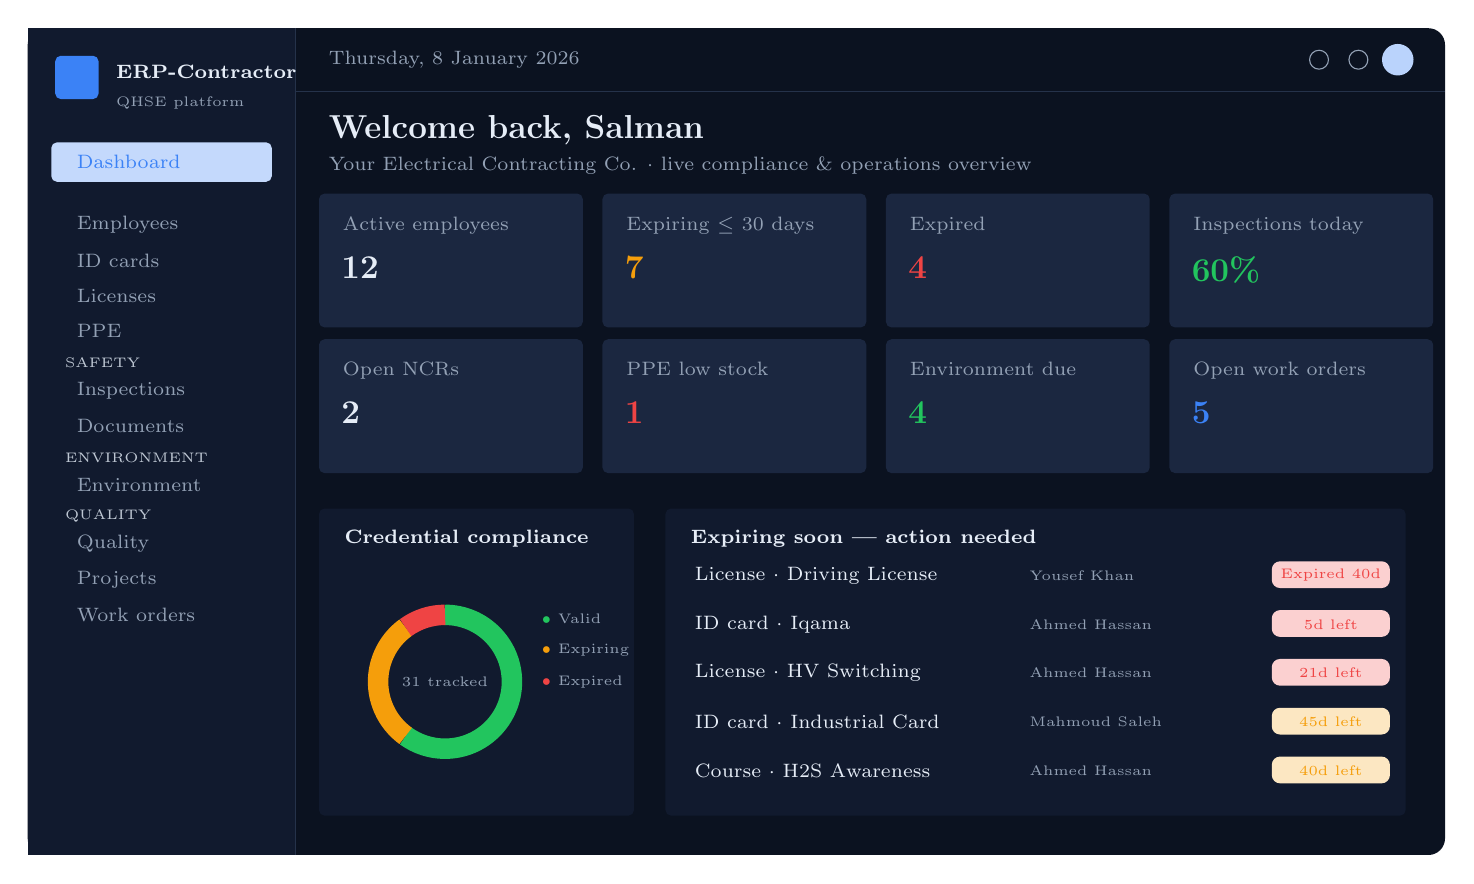
\begin{tikzpicture}
  % ---------- window ----------
  \fill[apbg,rounded corners=6pt] (0,0) rectangle (18,10.5);
  % ---------- sidebar ----------
  \fill[apsurface] (0,0) rectangle (3.4,10.5);
  \draw[apborder] (3.4,0)--(3.4,10.5);
  \fill[apblue,rounded corners=2pt] (0.35,9.6) rectangle ++(0.55,0.55);
  \node[anchor=west,text=aptext,font=\scriptsize\bfseries] at (1.0,9.95){ERP-Contractor};
  \node[anchor=west,text=apmuted,font=\tiny] at (1.0,9.55){QHSE platform};
  % active nav pill
  \fill[apblue!30,rounded corners=2pt] (0.3,8.55) rectangle ++(2.8,0.5);
  \node[anchor=west,text=apblue,font=\scriptsize] at (0.5,8.8){Dashboard};
  \foreach \yy/\nav in {8.0/Employees,7.55/ID cards,7.1/Licenses,6.65/PPE,5.9/Inspections,
                     5.45/Documents,4.7/Environment,3.95/Quality,3.5/Projects,3.05/Work orders}{
     \node[anchor=west,text=apmuted,font=\scriptsize] at (0.5,\yy){\nav};}
  \node[anchor=west,text=apmuted!60,font=\tiny] at (0.35,6.25){SAFETY};
  \node[anchor=west,text=apmuted!60,font=\tiny] at (0.35,5.05){ENVIRONMENT};
  \node[anchor=west,text=apmuted!60,font=\tiny] at (0.35,4.3){QUALITY};
  % ---------- top bar ----------
  \draw[apborder] (3.4,9.7)--(18,9.7);
  \node[anchor=west,text=apmuted,font=\scriptsize] at (3.7,10.1){Thursday, 8 January 2026};
  \foreach \x in {16.4,16.9}{\draw[apmuted] (\x,10.1) circle (0.12);}
  \fill[apblue!35] (17.4,10.1) circle (0.2);
  % ---------- heading ----------
  \node[anchor=west,text=aptext,font=\large\bfseries] at (3.7,9.2){Welcome back, Salman};
  \node[anchor=west,text=apmuted,font=\scriptsize] at (3.7,8.75)
        {Your Electrical Contracting Co. $\cdot$ live compliance \& operations overview};
  % ---------- KPI cards, row 1 ----------
  \kpicard{3.7}{6.7}{Active employees}{12}{aptext}
  \kpicard{7.3}{6.7}{Expiring $\leq$ 30 days}{7}{apamber}
  \kpicard{10.9}{6.7}{Expired}{4}{apred}
  \kpicard{14.5}{6.7}{Inspections today}{60\%}{apgreen}
  % ---------- KPI cards, row 2 ----------
  \kpicard{3.7}{4.85}{Open NCRs}{2}{aptext}
  \kpicard{7.3}{4.85}{PPE low stock}{1}{apred}
  \kpicard{10.9}{4.85}{Environment due}{4}{apgreen}
  \kpicard{14.5}{4.85}{Open work orders}{5}{apblue}
  % ---------- compliance donut ----------
  \fill[apsurface,rounded corners=2pt] (3.7,0.5) rectangle ++(4.0,3.9);
  \node[anchor=north west,text=aptext,font=\scriptsize\bfseries] at (3.9,4.25){Credential compliance};
  \coordinate (dc) at (5.3,2.2);
  \draw[apgreen,line width=0.26cm] ([shift={(90:0.85)}]dc) arc[start angle=90,end angle=-126,radius=0.85];
  \draw[apamber,line width=0.26cm] ([shift={(-126:0.85)}]dc) arc[start angle=-126,end angle=-234,radius=0.85];
  \draw[apred,line width=0.26cm]   ([shift={(-234:0.85)}]dc) arc[start angle=-234,end angle=-270,radius=0.85];
  \node[text=apmuted,font=\tiny] at (dc){31 tracked};
  \node[anchor=west,text=apmuted,font=\tiny] at (6.4,3.0){\textcolor{apgreen}{$\bullet$} Valid};
  \node[anchor=west,text=apmuted,font=\tiny] at (6.4,2.6){\textcolor{apamber}{$\bullet$} Expiring};
  \node[anchor=west,text=apmuted,font=\tiny] at (6.4,2.2){\textcolor{apred}{$\bullet$} Expired};
  % ---------- watchlist ----------
  \fill[apsurface,rounded corners=2pt] (8.1,0.5) rectangle ++(9.4,3.9);
  \node[anchor=north west,text=aptext,font=\scriptsize\bfseries] at (8.3,4.25){Expiring soon --- action needed};
  \foreach \ri/\kind/\nm/\dd/\cl in {%
      0/License $\cdot$ Driving License/Yousef Khan/Expired 40d/apred,
      1/ID card $\cdot$ Iqama/Ahmed Hassan/5d left/apred,
      2/License $\cdot$ HV Switching/Ahmed Hassan/21d left/apred,
      3/ID card $\cdot$ Industrial Card/Mahmoud Saleh/45d left/apamber,
      4/Course $\cdot$ H2S Awareness/Ahmed Hassan/40d left/apamber}{
    \node[anchor=west,text=aptext,font=\scriptsize] at (8.35,3.55-\ri*0.62){\kind};
    \node[anchor=west,text=apmuted,font=\tiny] at (12.6,3.55-\ri*0.62){\nm};
    \fill[\cl!25,rounded corners=3pt] (15.8,3.55-\ri*0.62-0.16) rectangle ++(1.5,0.34);
    \node[text=\cl,font=\tiny] at (16.55,3.55-\ri*0.62){\dd};}
\end{tikzpicture}}
\caption{The executive dashboard rendered in the application's dark theme, populated with the
platform's seeded demonstration data. Key indicators, the credential-compliance breakdown and the
``expiring soon'' watch-list are visible at a glance.}
\label{fig:dash}
\end{figure}

\subsection{People and Compliance}
Employee master records, with a profile view that gathers every linked ID card, license, course and
PPE issue in one place. PPE is tracked both as catalogue stock and as items issued to individuals
with an acknowledgment flag; inventory and storage are detailed in Section~\ref{sec:stock}.

\subsection{Safety}
Daily inspections are captured against a tagged asset (job site, vehicle or equipment). Selecting the
asset loads the appropriate checklist template; the module computes a score and a pass / conditional /
fail result and records proof of presence. A controlled document register manages ISO~45001 material
with full version history. The tag-based inspection workflow is detailed in Section~\ref{sec:nfc}.

\subsection{Environment}
A dedicated register for transformer cooling-oil pulls, staking returns and waste-removal schedules,
supporting the ``claimant'' extractor reports required by the client.

\subsection{Quality}
Non-conformance reports (NCRs) with root cause and corrective action, plus an audit register covering
internal, external and certification audits under ISO~9001.

\subsection{Projects and Executive Dashboard}
Projects carry progress and status; work orders are assigned to employees with priority and due dates
(work-order management is detailed in Section~\ref{sec:tasks}).
The dashboard (Figure~\ref{fig:dash}) aggregates indicators from every module into a single executive
overview for the CEO.

%=====================================================================
\section{NFC-Based Inspection System}\label{sec:nfc}
The safety module replaces unreliable paper logs with tag-based digital inspections that yield
verifiable proof of presence. Durable tags --- NFC, QR or barcode --- are fixed to every job site,
vehicle and item of equipment and registered against an asset record, so a single scan identifies
exactly what is being inspected.

\subsection{Tag-to-Asset Workflow}
\begin{enumerate}[leftmargin=1.4em]
  \item \textbf{Placement.} Tamper-resistant tags are mounted on trucks, cars, job-site boards and
        equipment; each is registered in \texttt{assets} with its identifier (license plate / site ID)
        and tag value.
  \item \textbf{Scan / select.} The officer scans (or selects) the tag; the application resolves it to
        the asset and auto-populates identifier, type and location.
  \item \textbf{Data segregation at source.} The asset type routes the record into one of two streams
        --- \emph{Site Safety} or \emph{Fleet} --- without any manual sorting.
  \item \textbf{Checklist.} A type-specific template loads; each line is marked OK, Not OK or N/A with
        an optional remark.
  \item \textbf{Proof of presence.} The inspector, timestamp and tag / asset identifier are recorded,
        giving an auditable record that the inspection physically took place.
\end{enumerate}

\begin{figure}[H]
\centering
\resizebox{\textwidth}{!}{%
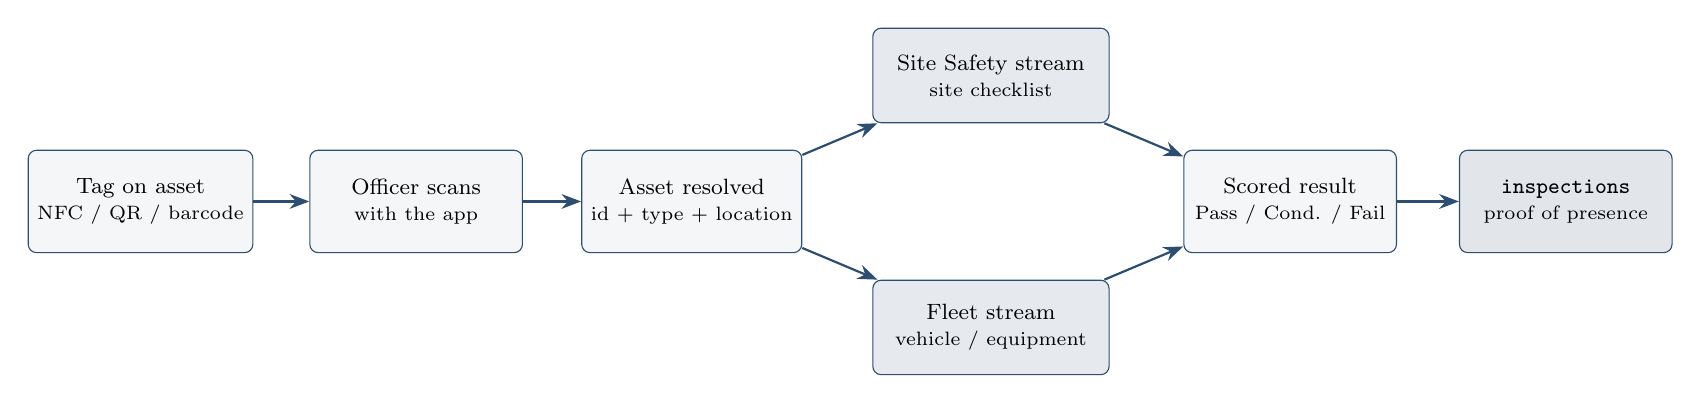
\begin{tikzpicture}[
  proc/.style={draw=reportblue,rounded corners=3pt,fill=reportblue!5,align=center,
               font=\footnotesize,minimum width=2.7cm,minimum height=1.3cm},
  br/.style={draw=reportblue,rounded corners=3pt,fill=reportblue!12,align=center,
             font=\footnotesize,minimum width=3.0cm,minimum height=1.2cm},
  arr/.style={-{Stealth[length=2.5mm]},thick,color=reportblue}]
  \node[proc] (tag)  at (0,0)      {Tag on asset\\ \scriptsize NFC / QR / barcode};
  \node[proc] (scan) at (3.5,0)    {Officer scans\\ \scriptsize with the app};
  \node[proc] (idn)  at (7.0,0)    {Asset resolved\\ \scriptsize id + type + location};
  \node[br]   (site) at (10.8,1.6) {Site Safety stream\\ \scriptsize site checklist};
  \node[br]   (veh)  at (10.8,-1.6){Fleet stream\\ \scriptsize vehicle / equipment};
  \node[proc] (score)at (14.6,0)   {Scored result\\ \scriptsize Pass / Cond. / Fail};
  \node[proc,fill=reportblue!14] (db) at (18.1,0) {\texttt{inspections}\\ \scriptsize proof of presence};
  \draw[arr] (tag)--(scan);
  \draw[arr] (scan)--(idn);
  \draw[arr] (idn) -- (site);
  \draw[arr] (idn) -- (veh);
  \draw[arr] (site) -- (score);
  \draw[arr] (veh) -- (score);
  \draw[arr] (score)--(db);
\end{tikzpicture}}
\caption{Tag-based inspection flow. The identifier captured at scan time routes each record into the
Site Safety or Fleet stream before it is scored and stored --- two operational views from one table.}
\label{fig:nfc}
\end{figure}

\subsection{Checklist Templates}
Three built-in, extensible templates cover the common cases:
\begin{itemize}
  \item \textbf{Site Safety} --- PPE worn correctly, work area barricaded, permit to work valid, earthing
        and isolation applied, tools inspected, emergency arrangements, housekeeping.
  \item \textbf{Vehicle} --- tyres and brakes, lights and indicators, warning beacon, first-aid and
        extinguisher, vehicle documents (Istimara), body and hydraulics, driver license valid.
  \item \textbf{Equipment} --- guards and safety devices, inspection sticker valid, earthing / RCD tested,
        no visible damage, operating manual available.
\end{itemize}

\subsection{Scoring and Result}
Let $n_{\mathrm{ok}}$ and $n_{\mathrm{no}}$ be the number of OK and Not-OK items (N/A items are
excluded). The score is
\[
s = \operatorname{round}\!\left( 100 \, \frac{n_{\mathrm{ok}}}{n_{\mathrm{ok}} + n_{\mathrm{no}}} \right)\%,
\]
and the result is \textsf{Pass} when $n_{\mathrm{no}} = 0$; \textsf{Conditional} when $n_{\mathrm{no}} > 0$
and $s \geq 70$; otherwise \textsf{Fail}. A failed inspection flags the asset for follow-up and can
raise a work order in the projects module.

\subsection{Two-Stream Reporting and Offline Operation}
Because the identifier captured at scan differs by asset type (site ID versus license plate), every
inspection lives in one table yet filters cleanly into a Site Safety view (by job site) and a Fleet
view (by vehicle / equipment) --- delivering the two platforms the department needs with no data
duplication. For disconnected field work, a mobile companion (future work, Section~\ref{sec:future})
caches inspections and synchronises on reconnection; each inspection is already stored as a structured
record with its full checklist.

%=====================================================================
\section{Stock, Inventory and PPE Storage}\label{sec:stock}
The platform manages both the \emph{store} of protective equipment and its \emph{allocation} to
individuals, giving a continuous, reconciled audit of who holds what and how much remains on hand.

\subsection{PPE Catalogue and Stock Levels}
Every catalogue item carries a category, unit, available sizes, a current stock level and a minimum
level. When stock reaches or falls below the minimum, the item is flagged and raises the dashboard
``PPE low stock'' indicator, prompting reorder.

\begin{table}[H]
\centering\small
\begin{tabular}{@{}l l l l r r l@{}}
\toprule
\textbf{Item} & \textbf{Category} & \textbf{Unit} & \textbf{Sizes} & \textbf{Stock} & \textbf{Min} & \textbf{Status} \\
\midrule
CAT-1 Insulating Helmet    & Head & pcs  & M/L/XL   & 4  & 6  & \textbf{Low} \\
Arc Flash Suit 8\,cal      & Body & set  & M/L/XL   & 9  & 4  & OK \\
Insulating Gloves Class 0  & Hand & pair & 9/10/11  & 12 & 8  & OK \\
Safety Glasses             & Eye  & pcs  & Std      & 40 & 15 & OK \\
Safety Boots S3            & Foot & pair & 40--44   & 18 & 10 & OK \\
Hi-Vis Vest                & Body & pcs  & M/L/XL   & 30 & 12 & OK \\
\bottomrule
\end{tabular}
\caption{Seeded PPE catalogue. An item is flagged \textbf{Low} when $\text{stock} \leq \text{minimum}$;
here the CAT-1 helmet (4 of a 6 minimum) drives the low-stock alert.}
\end{table}

\subsection{Issue, Acknowledgment and Return}
When equipment is issued, the system records the employee, item, size, quantity, issue date and a
re-test / expiry date, and requires an \emph{acknowledgment} --- the worker signs for the item. Each
issue carries a status: \textsf{Issued}, \textsf{Returned}, \textsf{Lost} or \textsf{Expired}. An
employee's profile shows the complete history of equipment they hold, and any dated item (for example
insulating gloves requiring periodic re-test) flows into the compliance engine exactly like an
expiring credential.

\begin{figure}[H]
\centering
\resizebox{0.95\textwidth}{!}{%
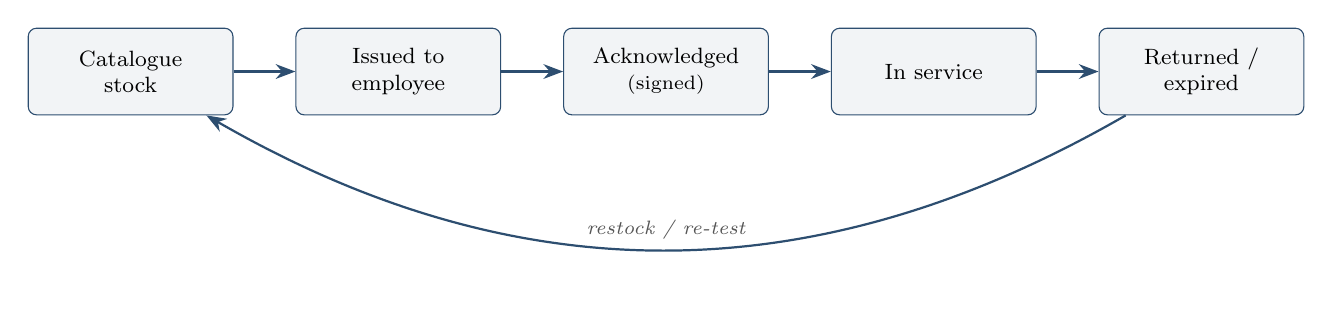
\begin{tikzpicture}[
  st/.style={draw=reportblue,rounded corners=3pt,fill=reportblue!6,align=center,
             font=\footnotesize,minimum width=2.6cm,minimum height=1.1cm},
  arr/.style={-{Stealth[length=2.5mm]},thick,color=reportblue}]
  \node[st] (stock) at (0,0)    {Catalogue\\ stock};
  \node[st] (issue) at (3.4,0)  {Issued to\\ employee};
  \node[st] (ack)   at (6.8,0)  {Acknowledged\\ \scriptsize (signed)};
  \node[st] (use)   at (10.2,0) {In service};
  \node[st] (end)   at (13.6,0) {Returned /\\ expired};
  \draw[arr] (stock)--(issue);
  \draw[arr] (issue)--(ack);
  \draw[arr] (ack)--(use);
  \draw[arr] (use)--(end);
  \draw[arr] (end) to[bend left=30] node[above,font=\scriptsize\itshape,color=inkgray]{restock / re-test} (stock);
\end{tikzpicture}}
\caption{PPE lifecycle. Returned items replenish stock; dated items re-enter the compliance engine at
their re-test date.}
\end{figure}

\subsection{Equipment Storage and Asset Registry}
Beyond consumable PPE, stored equipment --- generators, cable rigs, tools --- is registered in the
\texttt{assets} table with its own tag, storage location and status. Stored items are therefore
inventoried, inspectable through the same NFC / QR workflow (Section~\ref{sec:nfc}), and traceable to a
physical location at all times.

\subsection{Inventory Integrity}
Because stock levels and issue history share one relational store, the on-hand count and the allocation
record reconcile automatically --- there is no separate spreadsheet to drift out of sync. Every stock
adjustment and issue is written to the \texttt{audit\_log}, providing a defensible inventory trail.

%=====================================================================
\section{Work-Order and Task Management}\label{sec:tasks}
Field and office work is coordinated through work orders (tasks) attached to projects, turning the
platform from a passive record-keeper into an active operational coordination tool.

\subsection{Task Structure}
Each work order carries a parent project, a title, an assignee drawn from the employee master, a priority
(\textsf{Low}, \textsf{Medium}, \textsf{High}, \textsf{Urgent}), a status, a due date and a free-text
description. Because the assignee is a real employee record, that person's licenses, competencies and
issued PPE are one click away when work is allocated --- a supervisor can avoid assigning, say,
high-voltage work to someone whose HV license has lapsed.

\subsection{Lifecycle and States}
A work order moves through four states. A task whose due date has passed while it is not yet
\textsf{Done} is additionally flagged \emph{overdue} in red, reusing the compliance colour language so
attention is drawn consistently across the whole platform.

\begin{figure}[H]
\centering
\resizebox{0.72\textwidth}{!}{%
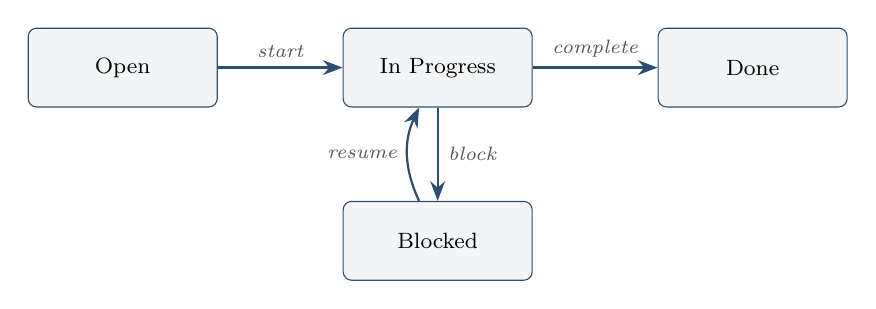
\begin{tikzpicture}[
  s/.style={draw=reportblue,rounded corners=3pt,fill=reportblue!6,align=center,
            font=\footnotesize,minimum width=2.4cm,minimum height=1.0cm},
  arr/.style={-{Stealth[length=2.5mm]},thick,color=reportblue},
  lbl/.style={font=\scriptsize\itshape,color=inkgray}]
  \node[s] (open)  at (0,0)   {Open};
  \node[s] (prog)  at (4,0)   {In Progress};
  \node[s] (done)  at (8,0)   {Done};
  \node[s] (block) at (4,-2.2){Blocked};
  \draw[arr] (open) -- node[lbl,above]{start} (prog);
  \draw[arr] (prog) -- node[lbl,above]{complete} (done);
  \draw[arr] (prog) -- node[lbl,right]{block} (block);
  \draw[arr] (block) to[bend left=25] node[lbl,left]{resume} (prog);
\end{tikzpicture}}
\caption{Work-order state model. Priority sets the colour (Urgent / High red, Medium amber, Low grey);
an overdue task is flagged regardless of priority.}
\end{figure}

\subsection{Priority and Overdue Detection}
Priority is colour-coded for instant triage, and due dates reuse the day-difference logic of the
compliance engine: a task with due date $d < 0$ that is not \textsf{Done} is overdue. The dashboard's
``Open work orders'' indicator counts every task not yet \textsf{Done}.

\subsection{Cross-Module Origination}
Crucially, work orders are not created only by hand --- they close the loop between detection and action:
\begin{itemize}
  \item a \textbf{failed inspection} (Section~\ref{sec:nfc}) raises a corrective work order against the asset;
  \item an \textbf{open NCR} in quality spawns corrective-action tasks with owners and due dates;
  \item a \textbf{low-stock PPE} item can trigger a reorder task.
\end{itemize}

\subsection{Executive Roll-Up}
Individual tasks aggregate upward: project progress is derived from task completion, and the executive
dashboard summarises open work, overdue items and completion rates so management sees operational health
without chasing individual updates.

%=====================================================================
\section{Compliance and Expiry Engine}
\subsection{Status Classification}
Every credential with an expiry date is classified daily. Let $d$ be the number of days until expiry.
The status is
\[
\text{status}(d)=
\begin{cases}
\textsf{expired}  & d < 0,\\[2pt]
\textsf{critical} & 0 \leq d \leq 30,\\[2pt]
\textsf{warning}  & 30 < d \leq 90,\\[2pt]
\textsf{valid}    & d > 90,
\end{cases}
\]
rendered as red, red, amber and green respectively. The thresholds echo the client's escalating
notification points.

\subsection{Watch-list and Alerts}
A single union query gathers every dated credential --- ID cards, licenses, courses and PPE --- computes
$d$, and sorts ascending. The result drives the dashboard watch-list, the alert badge count, and the
alerts panel, converting a reactive risk (a lapsed credential discovered too late) into a managed,
visible process.

%=====================================================================
\section{Data Interoperability}
Because the existing workflow is spreadsheet-based, every module exports to a formatted Excel workbook.
Personnel and credential tables additionally support import: column headers are matched
case-insensitively to database fields, and employees are \emph{upserted} by \texttt{emp\_id} so a weekly
refresh updates existing people rather than duplicating them. The import path acts as a validation
gate rather than a blind copy, protecting the integrity of the single source of truth.

%=====================================================================
\section{Security, Access and Data Ownership}
\begin{itemize}
  \item \textbf{Local ownership.} Data lives in one SQLite file under the user's control; there is no
        cloud service and no third party with a copy.
  \item \textbf{Isolation.} The interface reaches data only through the single preload bridge; it holds
        no database or file-system handles.
  \item \textbf{Credentials.} Application logins are stored salted and hashed (scrypt), never in plain text.
  \item \textbf{Audit trail.} The append-only \texttt{audit\_log} records who changed what and when.
  \item \textbf{Roles.} A role field is retained on every account for future least-privilege policies;
        the delivered configuration grants full edit to all operators by request.
\end{itemize}

%=====================================================================
\section{Deployment and Operation}
\begin{table}[H]
\centering\small
\begin{tabular}{@{}l l@{}}
\toprule
\textbf{Concern} & \textbf{Detail} \\
\midrule
Launch          & \texttt{npm run dev}, or the bundled desktop launch shortcut \\
Runtime         & Electron desktop window; Vite dev server on a dedicated local port \\
Data location   & Per-user application-data directory (single \texttt{.sqlite} file) \\
Backup          & Copy the single \texttt{.sqlite} file \\
Offline         & Fully functional with no network connection \\
\bottomrule
\end{tabular}
\caption{Operational summary.}
\end{table}

%=====================================================================
\section{Verification and Results}
\begin{table}[H]
\centering\small
\begin{tabular}{@{}l l@{}}
\toprule
\textbf{Check} & \textbf{Result} \\
\midrule
Front-end production build            & Compiles cleanly (2{,}205 modules, 0 errors) \\
Database schema and seeding           & 12 employees and all module data created \\
Authentication                        & Valid login accepted; invalid rejected \\
KPI aggregation                        & Correct counts (e.g.\ 7 expiring, 4 expired) \\
Compliance union query                 & Correct day-to-expiry and ordering \\
Create / read / update / delete        & Verified across modules \\
Excel import / export                  & Round-trips verified \\
Application boot                       & Launches, initialises database, no errors \\
Persistence                            & Data survives restart (no re-seed) \\
\bottomrule
\end{tabular}
\caption{Verification summary for version~1.0.}
\end{table}

%=====================================================================
\section{Limitations and Future Work}\label{sec:future}
\subsection{Current Limitations}
\begin{itemize}
  \item \textbf{Physical NFC capture.} The data model is tag-ready, but live NFC taps in the field require
        a mobile companion; the desktop client uses tag-ID / selection and manual entry.
  \item \textbf{Packaged binary.} The system runs from the development launcher; a signed, double-click
        application bundle is a straightforward next step.
  \item \textbf{Single workstation.} The database is local to one machine; concurrent multi-user access
        is not yet supported.
  \item \textbf{In-app notifications only.} Expiry alerts surface inside the application; email, SMS and
        Teams delivery are not yet wired.
  \item \textbf{English interface.} An Arabic (right-to-left) interface is not yet provided.
\end{itemize}

\subsection{Roadmap}
The architecture is deliberately extensible: one relational store and one uniform data channel mean new
modules and integrations attach without disturbing what already works. Growth is planned in three phases.

\begin{table}[H]
\centering\small
\begin{tabular}{@{}l l p{8.2cm}@{}}
\toprule
\textbf{Phase} & \textbf{Theme} & \textbf{Key deliverables} \\
\midrule
Phase 2 & Field \& mobility &
  Mobile companion for live NFC / QR taps with offline caching and sync; camera-based scanning;
  signed, double-click desktop binary; Arabic (RTL) localisation. \\[2pt]
Phase 3 & Automation \& integration &
  Scheduled PDF / Excel client reports emailed automatically; email / SMS / Teams expiry alerts;
  granular role-based access (least privilege); integration hooks to government portals
  (Iqama / Muqeem, Municipality) and payroll / HRIS; one-click weekly client data export. \\[2pt]
Phase 4 & Intelligence \& scale &
  Predictive safety analytics that flag high-risk assets and sites from inspection history; optional
  encrypted multi-device sync and backup; forecasting dashboards; e-signature for PPE acknowledgment
  and applications; audit-ready compliance report packs. \\
\bottomrule
\end{tabular}
\caption{Phased roadmap. Each phase builds on the delivered version~1.0 core without re-architecting it.}
\end{table}

\subsection{Extensibility Note}
Because every module is a table plus a configuration entry, adding a new register --- for example a
training-matrix or a permit-to-work log --- is largely declarative. The retained per-account role field
activates least-privilege access whenever the organisation is ready, and the Excel import / export path
provides an immediate bridge to any external system pending a deeper integration.

%=====================================================================
\section{Conclusion}
ERP-Contractor replaces a fragile, spreadsheet-based process with a single, owned, offline platform that
unifies safety, environment, quality, personnel and project operations. Its relational core, proactive
compliance engine and department-aligned modules convert scattered records into a coherent, auditable
system --- delivering immediate operational visibility while remaining entirely under the user's control.

\appendix
\section{Key Performance Indicators}
\begin{table}[H]
\centering\small
\begin{tabular}{@{}l p{8.5cm}@{}}
\toprule
\textbf{Indicator} & \textbf{Definition} \\
\midrule
Active employees      & Count of employees with status \textsf{Active} \\
Expiring $\leq$ 30 d  & Credentials with $0 \leq d \leq 30$ \\
Expired               & Credentials with $d < 0$ \\
Inspections today     & Completed today $\div$ active sites and vehicles \\
Open NCRs             & Non-conformance reports not \textsf{Closed} \\
PPE low stock         & Catalogue items at or below minimum level \\
Environment due       & Environmental records not \textsf{Completed} \\
Open work orders      & Tasks not \textsf{Done} \\
\bottomrule
\end{tabular}
\caption{Dashboard indicators and their definitions.}
\end{table}

\end{document}
